\documentclass[handout]{beamer}

\usepackage{mathtools}
\usepackage{graphicx}

\usetheme{Warsaw}

\AtBeginSection[]
{
  \begin{frame}
    \frametitle{Table of Contents}
    \tableofcontents[currentsection]
  \end{frame}
}

\title[compressed SDF rendering]{GPU-efficient and compressed representation of
implicit surfaces for real-time rendering}
\author[Debussche, Jambon]{Marius DEBUSSCHE\inst{1}, Clément JAMBON\inst{1} \\
Supervised by Tamy BOUBEKEUR\inst{2}}
\date[2021-2022]
{2021-2022}
\institute[Ecole polytechnique]
{
  \inst{1}%
  Advanced Program \textit{Image, Vision and Machine Learning}\newline
  \'Ecole polytechnique \\
  \inst{2}%
  Adobe Research, \'Ecole polytechnique
}
\subject{INF515}

\begin{document}

\begin{frame}[plain]\titlepage\end{frame}

\begin{frame}
  \frametitle{Why Signed Distance Fields ?}
  \begin{figure}
    \centering
    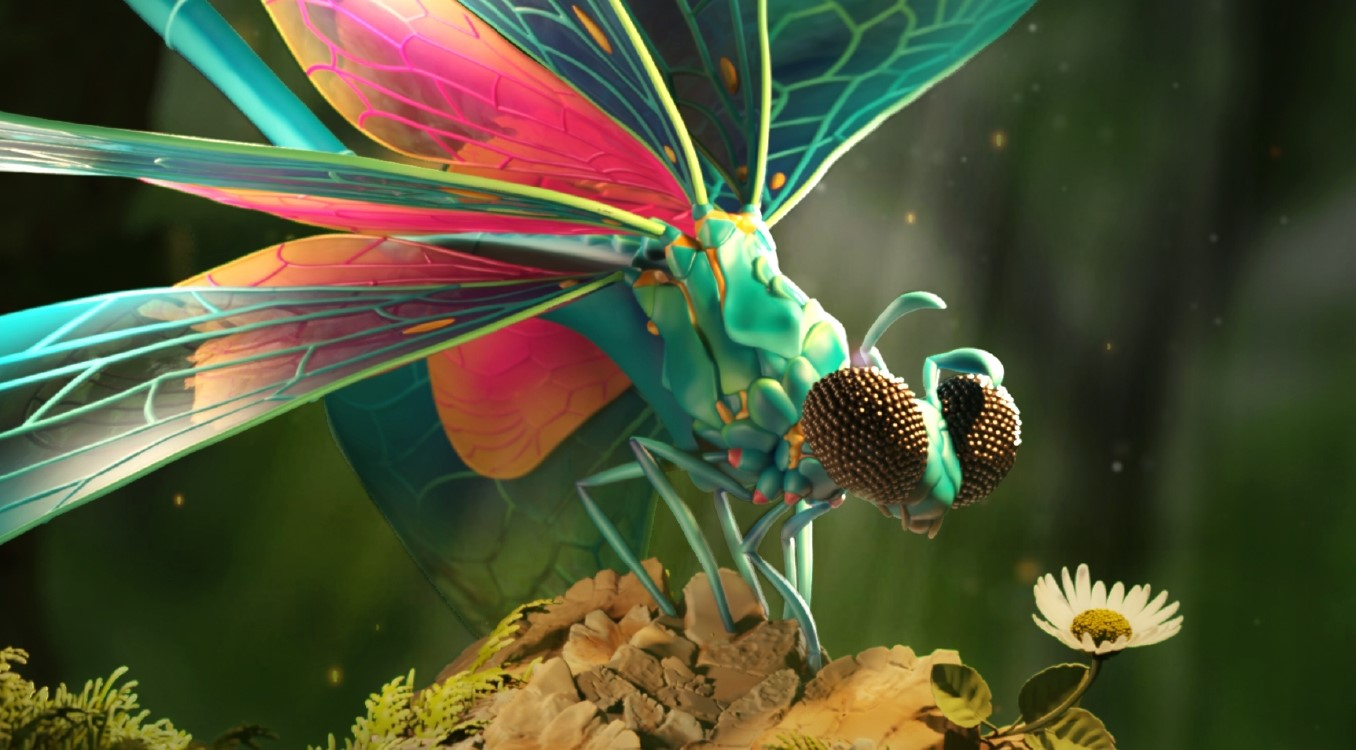
\includegraphics[width=0.9\textwidth]{figures/medium.jpg}
    \caption{Screenshot of a render in Adobe Medium}
    \label{fig:medium}
  \end{figure}
\end{frame}

\section{Preliminary works}

\subsection{Rendering SDFs}
\begin{frame}
  \frametitle{The rendering algorithm}
  \begin{figure}
    \centering
    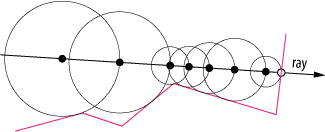
\includegraphics[width=0.5\textwidth]{figures/raymarching-0.png}
    \caption{The ray marching algorithm}
    \label{fig:ray-marching}
  \end{figure}
\end{frame}

\begin{frame}
  \frametitle{Our first results}
  \begin{figure}
    \centering
    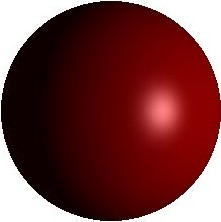
\includegraphics[width=0.4\textwidth]{figures/ray_marching_phong.JPG}
    \caption{Perfect sphere rendered with the ray marching algorithm, with Phong Shading}
    \label{fig:sphere-phong}
  \end{figure}
\end{frame}

\subsection{Discretizing SDFs}

\begin{frame}
  \frametitle{Major issues}

  \begin{itemize}
    \item With this approach, the scene has to be mathematically describes in the GPU, which is realistically impossible for large scenes.
    \item How to send the scene information to the GPU ? We can't send functions, let alone CSG trees of every item of the scene.
    \item We can't render the entire scene at once, so we need to find a way to render each object separately.
  \end{itemize} 
  
\end{frame}

\begin{frame}
  \frametitle{The state of the art: Claybook}
  \begin{figure}
    \centering
    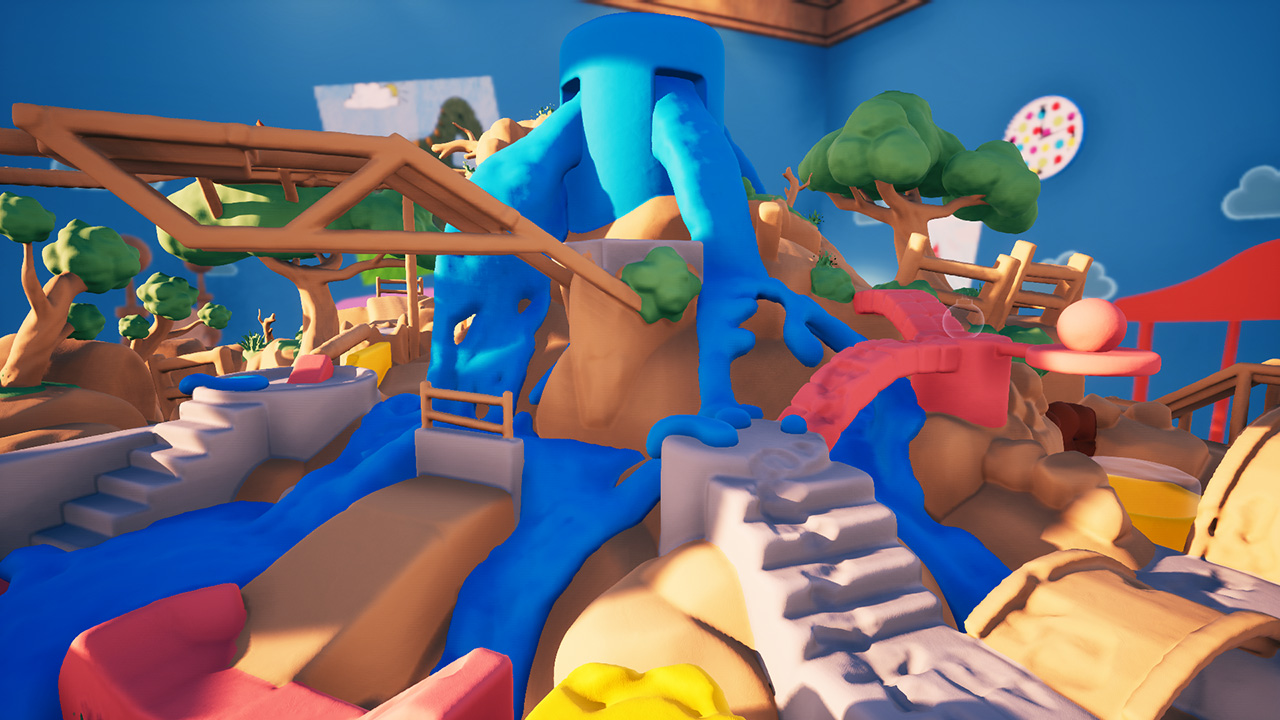
\includegraphics[width=0.8\textwidth]{figures/claybook.jpg}
    \caption{Screenshot of the game Claybook}
    \label{fig:claybook}
  \end{figure}
\end{frame}

\begin{frame}
  \frametitle{The state of the art: Claybook}
  \begin{itemize}
    \item Every object in the scene is rendered with discretized SDFs which were previously generated by compute shaders.
    \item The distance function is stored on one byte, varying from -4 to +4 texture units of distance.
    \item The scene is dynamic, so the textures that store the SDFs have to be updated.
  \end{itemize}
\end{frame}

\subsection{Our implementation}
\begin{frame}
  \frametitle{Basic render with Phong Shading}
  \begin{figure}
    \centering
    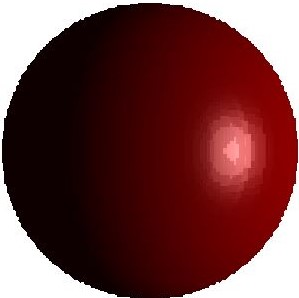
\includegraphics[width=0.4\textwidth]{figures/discretized_sdf_256.JPG}
    \caption{Render of a discretized signed distance field with Phong shading and low resolution}
    \label{fig:discretized-sdf-implemetation}
  \end{figure}
\end{frame}

\begin{frame}
  \frametitle{Ameliorations}
  \begin{itemize}
    \item We already passed the normals through a 3D texture. (We actually only need one texture becaude we can use the 4 RGBA channels)
    \item We need to improve the resolution by setting the distance function relative to the density of the SDF texture.
    \item We need to sample the SDF textures in compute shaders to allow for real time generation and display.
  \end{itemize}
  
\end{frame}

\section{Representing SDFs}
\subsection{Previous works}
\begin{frame}
  \frametitle{Adaptively Sampled Distance Fields}
  \begin{figure}
    \centering
    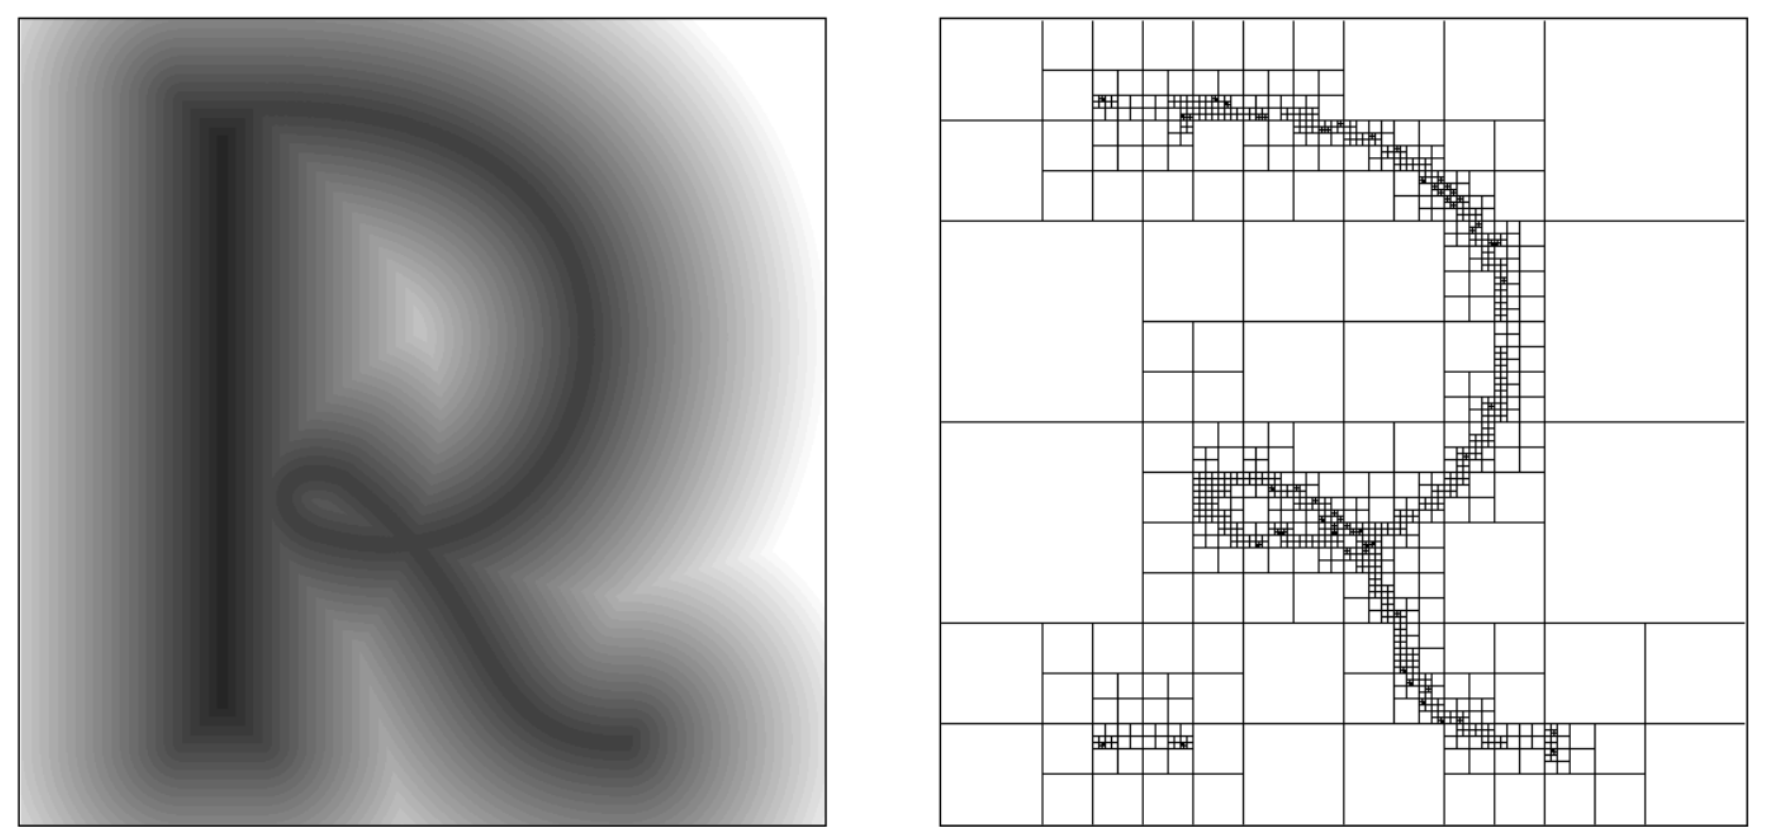
\includegraphics[width=0.95\textwidth]{figures/asdf.png}
    \caption{2d representation of ASDF}
    \label{fig:asdf}
  \end{figure}
  \scriptsize Borrowed from: \textit{Adaptively Sampled Distance Fields: A General Representation of Shape for Computer Graphics}
\end{frame}
\begin{frame}
  \frametitle{Gigavoxels}
  \begin{figure}
    \centering
    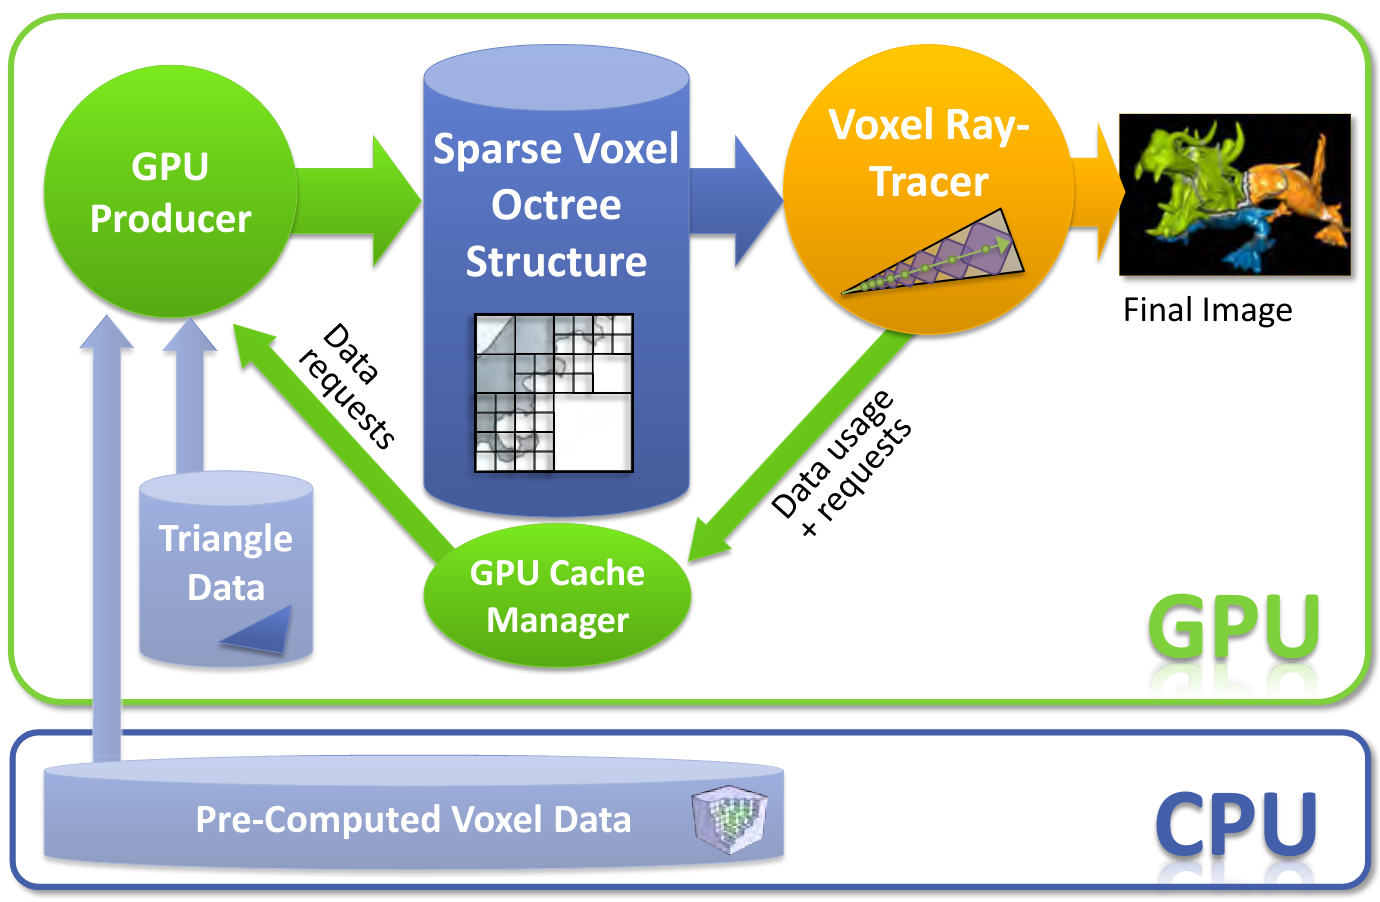
\includegraphics[width=0.65\textwidth]{figures/gigavoxels-pipeline.png}
    \caption{\textit{Gigavoxels} full rendering pipeline}
    \label{fig:gigavoxels-pipeline}
  \end{figure}
  \scriptsize Borrowed from: \textit{GigaVoxels: A Voxel-Based Rendering Pipeline For Efficient Exploration Of Large And Detailed Scenes}
\end{frame}
\begin{frame}
  \frametitle{Gigavoxels}
  \begin{figure}
    \centering
    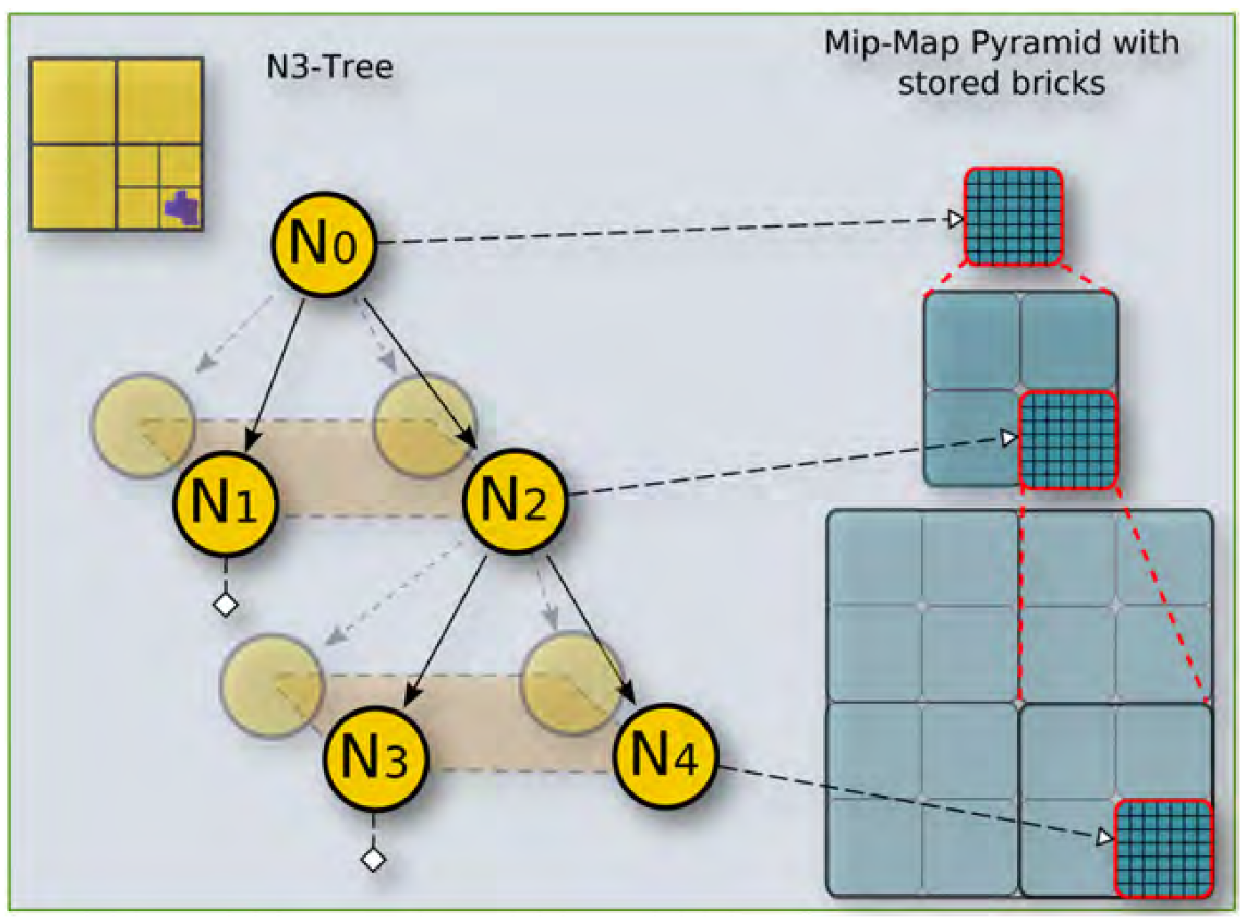
\includegraphics[width=0.65\textwidth]{figures/gigavoxels-tree.png}
    \caption{Sparse voxel octree datastructure used introduced in \textit{Gigavoxels}}
    \label{fig:gigavoxels-datastructure}
  \end{figure}
  \scriptsize Borrowed from: \textit{GigaVoxels: A Voxel-Based Rendering Pipeline For Efficient Exploration Of Large And Detailed Scenes}
\end{frame}
\begin{frame}
  \frametitle{Hash-based methods}
  \begin{figure}
    \centering
    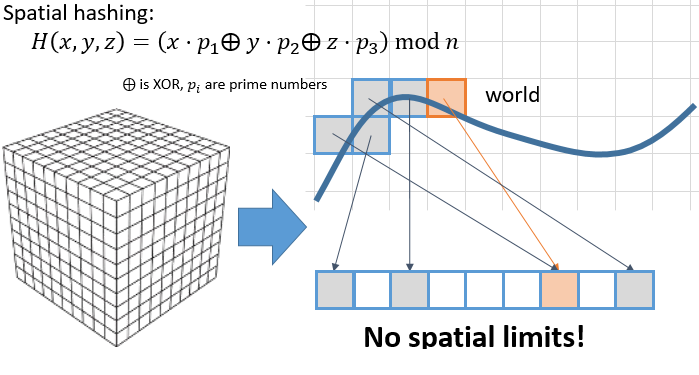
\includegraphics[width=0.95\textwidth]{figures/voxel-hashing.png}
    \caption{Voxel hashing architecture}
    \label{fig:voxel-hashing}
  \end{figure}
  \scriptsize Borrowed from: \textit{Real-time 3D Reconstruction at Scale using Voxel Hashing}
\end{frame}

\subsection{Dictionary-based sampling of SDFs}
\begin{frame}
  \frametitle{Inspiration: Compression and Rendering of Point Clouds}
  \begin{figure}
    \centering
    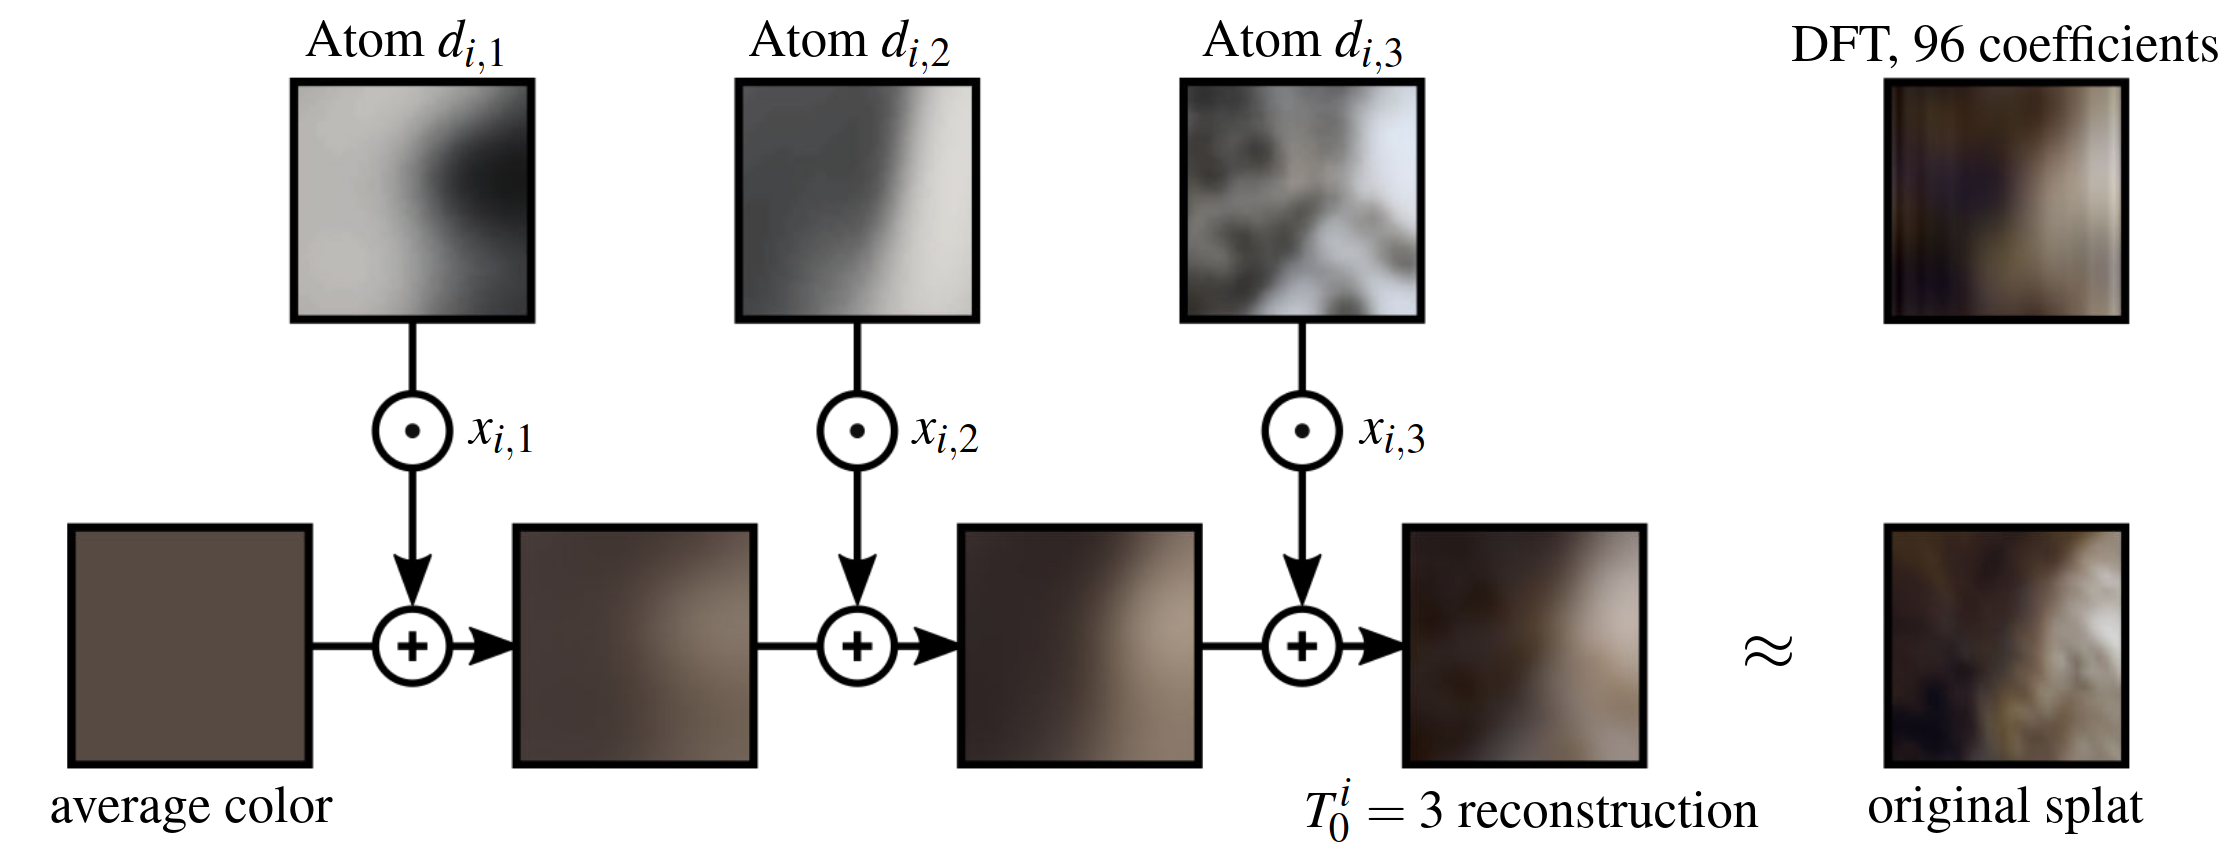
\includegraphics[width=0.95\textwidth]{figures/point-cloud-splat.png}
    \caption{Sparse coding of point cloud texture splats}
    \label{fig:spoint-cloud-splat}
  \end{figure}
  \scriptsize Borrowed from: \textit{Compression and Rendering of Textured Point Clouds via Sparse Coding}
\end{frame}
\begin{frame}
  \frametitle{Proposed representation}
  \begin{figure}
    \centering
    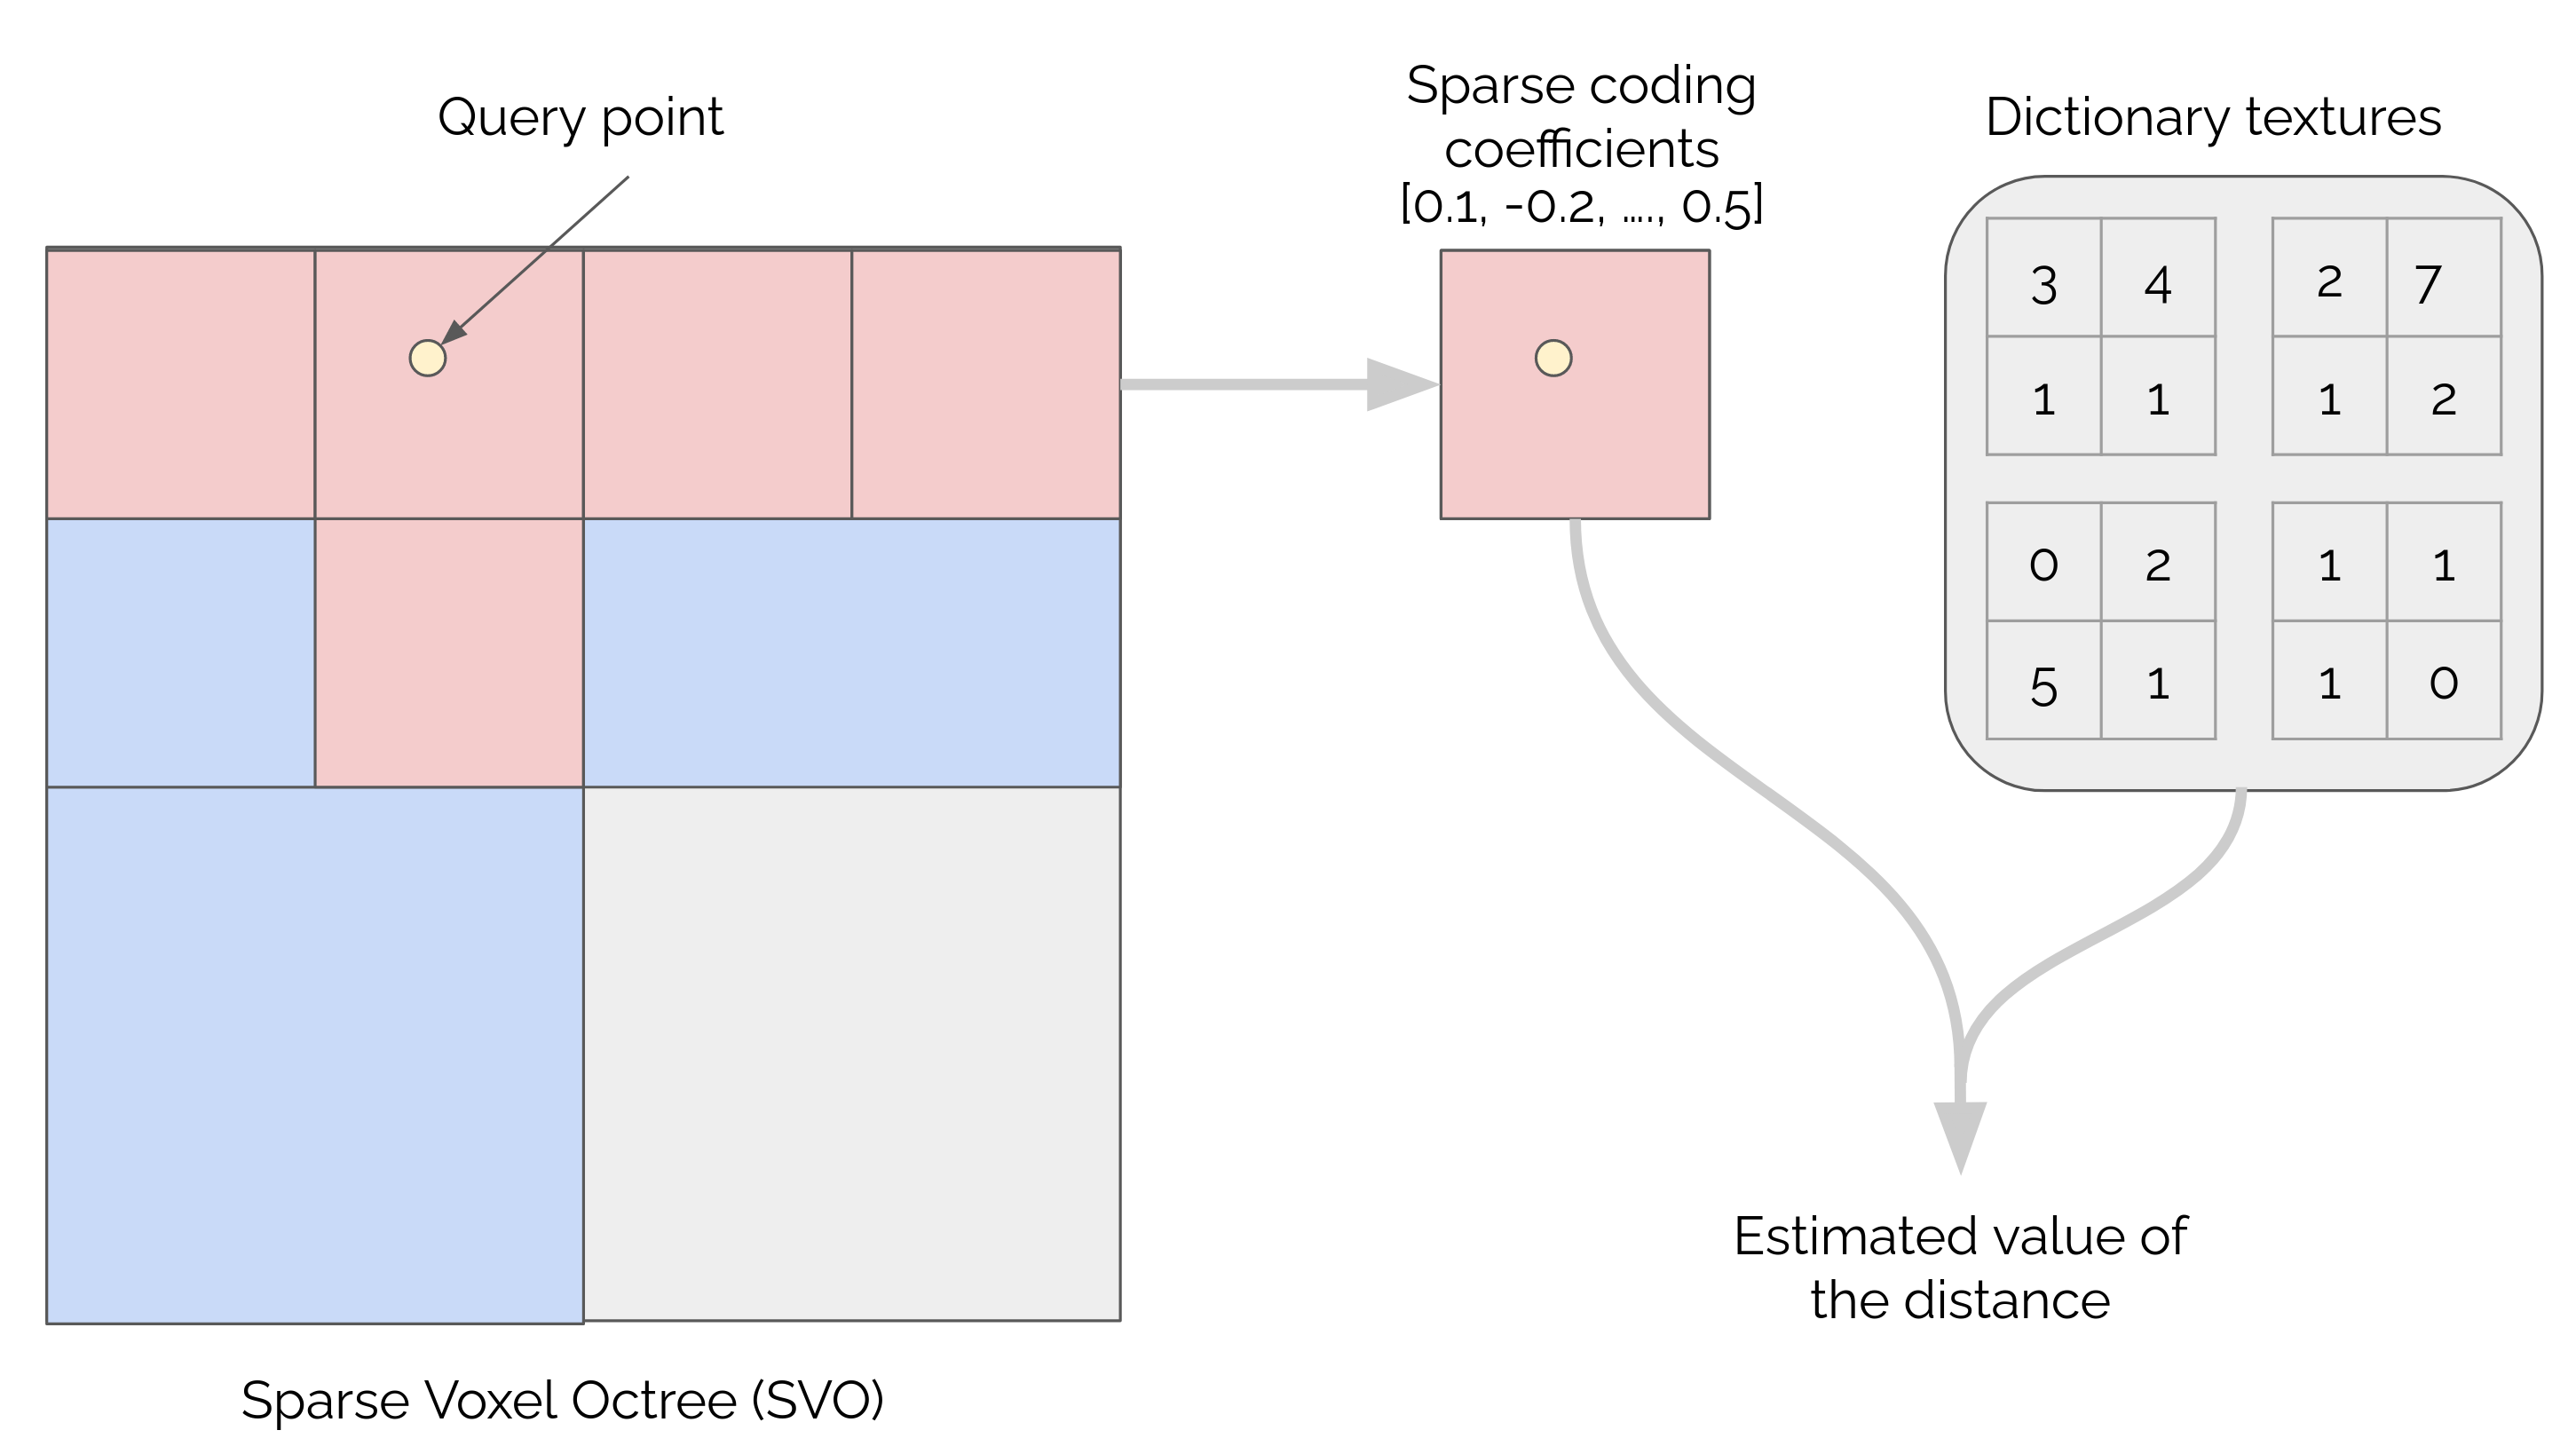
\includegraphics[width=0.95\textwidth]{figures/sparse-coding-sdf.png}
    \caption{Proposed dictionary-based representation of the SDF}
    \label{fig:sparse-coding-sdf}
  \end{figure}
\end{frame}

\subsection{Neural representations of SDFs}
\begin{frame}
  \frametitle{Representing SDF locally as learned features}
  \begin{figure}
    \centering
    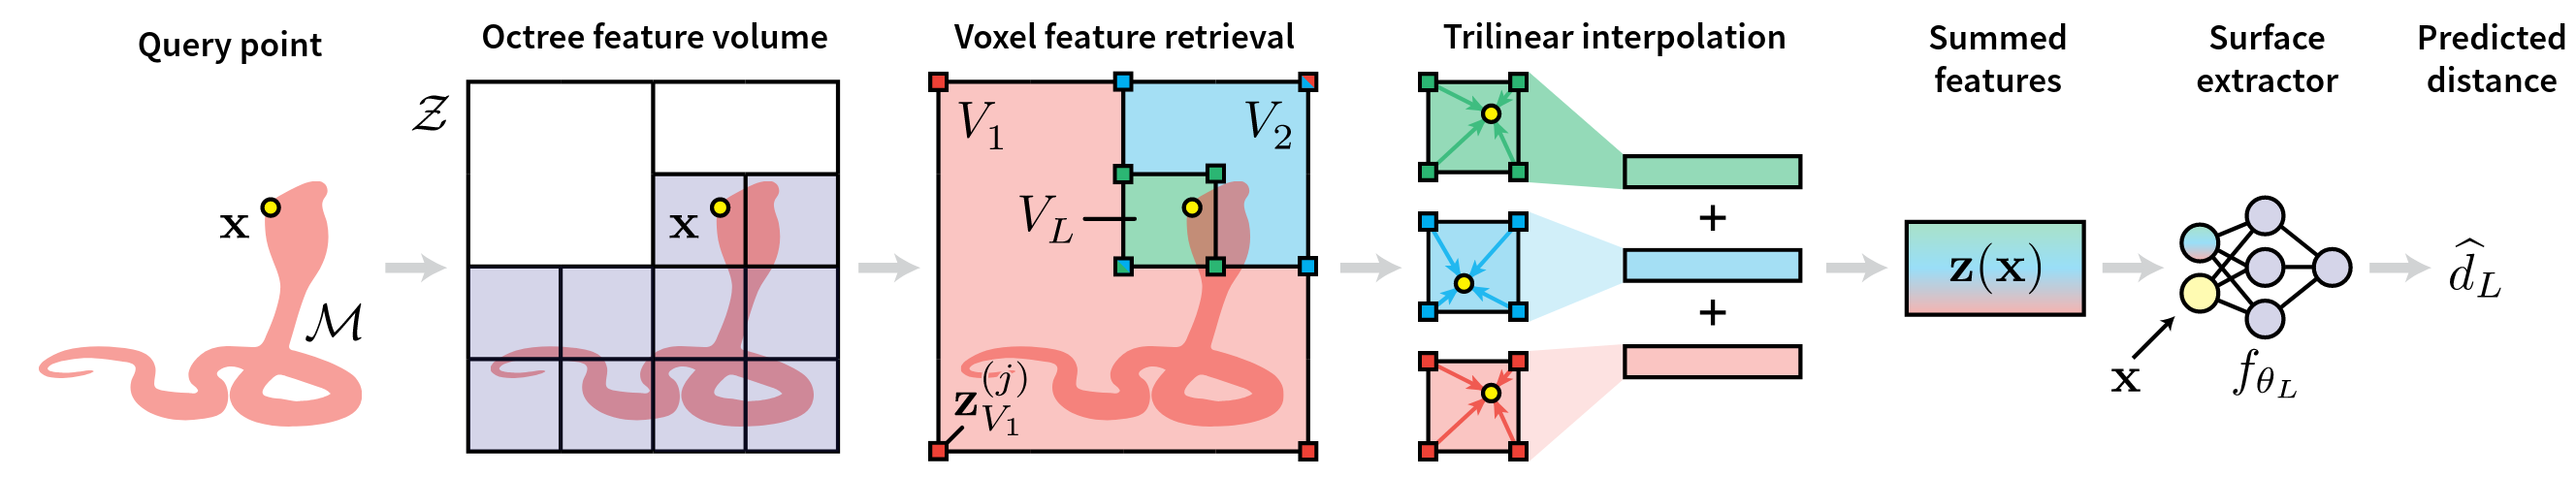
\includegraphics[width=0.95\textwidth]{figures/neural-sdf.png}
    \caption{Architecture proposed in \textit{Neural Geometric Level of Detail: Real-time Rendering with Implicit 3D Shapes}}
    \label{fig:neural-sdf}
  \end{figure}
\end{frame}


\section{Generating SDFs}

\subsection{Goals}

\begin{frame}
  \frametitle{List of ideal goals for SDF generation}
  \begin{itemize}
    \item Real-time rendering is our main constraint.
    \item Flexible solution, able to render complex objects with CSG trees.
    \item Render objects of different scale in the same scene.
    \item Maybe a loading/streaming system to allow for real time loading of large scenes.
  \end{itemize}
\end{frame}

\end{document}